%!TEX root = ../nwoods_thesis.tex

% chktex-file 15

\chapter{The Standard Model}

\section{Introduction}

The standard model (SM) is a theory---or rather, set of several related theories---that encapsulates everything we currently know about matter and its interactions at a fundamental level.
This is a remarkable claim: in the particle physicist's reductionist worldview, subatomic particle interactions are the substrate underlying the rest of reality, with all other physics, and by extension everything else, arising as emergent properties.
Of course, the SM is a remarkable theory, making detailed predictions on a wide range of topics that have matched data in essentially every experiment over roughly four decades.
The small number of known phenomena outside the SM are topics on which it makes no prediction; it is fully self-consistent and on the topics it covers, it is consistent with data to the precision achievable by any experiment to date.
It is arguably the best-confirmed theory in the history of science despite making some of the boldest, broadest, and most precise predictions.
It is generally believed that future advances will add to it, explain its free parameters, or find some underlying structure, not contradict it.

The following sections give a general overview of the SM and related topics that serve as background material for the four-lepton processes described in more detail in the following chapters.
This will include discussions of the particle content of the SM and the gauge structure that leads to particle interactions, the spontaneous symmetry breaking mechanism that leads to the specific structure of the electroweak sector of the SM, diboson processes, and the SM's limitations and how they might be addressed.
Some details will also be given about the proton-proton interactions used to probe particle interactions at high energies.
More complete information may be found in a number of texts, including Refs.~\cite{Griffiths:111880,Halzen:1984mc,barger1997collider,Peskin:1995ev,Donoghue:238727}.
Unless otherwise stated, everything that follows uses units such that $c = \hbar = 1$, where $c$ is the speed of light and $\hbar$ is the reduced Planck's constant $\hbar = h / 2\pi$.



\section{Matter and Force}

In the SM, matter is made of fermions (particles with half-integer spin; in fact all SM fundamental fermions have spin $\frac{1}{2}$) which interact by exchanging gauge bosons (integer spin; spin 1 for the SM force carriers).
Table~\ref{tab:sm} lists the fundamental particles and some of their properties.
With the exception of the neutral bosons, all particles have a corresponding antiparticle which is the same except that all its quantum numbers have opposite sign.
The fermions come in two broad categories, leptons and quarks.
All the quarks and half the lepton types carry electric charge and are therefore subject to interactions through the electromagnetic force, described by quantum electrodynamics (QED).
In a QED interaction, two charged particles exchange a photon, which carries the momentum transferred from one charged particle to the other.
The photon is a spin-1 gauge boson that is electrically neutral itself and massless, explaining why electromagnetic forces are long-range.
Because it is so simple, QED was the first theory of fundamental force to be worked out in detail, and it served as the template for the theories of the other forces.
The Feynman diagram at leading order (LO) in perturbation theory for a simple QED interaction, the so-called Drell-Yan process, in which a fermion-antifermion pair ($\Pf\Paf$, where {\Pf} can be any charged fermion) annihilates and produces a different pair ($\Pf'\Paf'$) is shown in in Fig.~\ref{fig:drellYanDiagram}.
Our conventions for Feynman diagrams will be that time increases from left to right, fermions are straight lines with an arrow whose direction differentiates fermions (arrow points right) from antifermions (arrow points left), and photons are shown as wavy lines.

\begin{figure}[htbp]
  \vspace{1em}
  \begin{center}
    \begin{fmffile}{drellYanDiagram}
      \begin{fmfgraph*}(0.6,0.3) % chktex 36
        \fmfleft{i1,i2}
        \fmfright{o1,o2}
        \fmflabel{$\Pf$}{i1}
        \fmflabel{$\Paf$}{i2}
        \fmflabel{$\Paf'$}{o1}
        \fmflabel{$\Pf'$}{o2}
        \fmf{fermion}{i1,v1,i2}
        \fmf{fermion}{o1,v2,o2}
        \fmf{photon,label=$\Pa$}{v1,v2}
      \end{fmfgraph*}
    \end{fmffile}
    \vspace{1em}
    \caption[Feynman diagram of an electromagnetic Drell-Yan interaction]{
        Feynman diagram of fermion-antifermion scattering through an electromagnetic interaction, resulting in another fermion-antifermion pair.
        This is also known as a Drell-Yan process.
        At center-of-mass energies near and above the {\PZ} boson mass, {\PZ}-{\Pa} interference becomes nonnegligible.
      }\label{fig:drellYanDiagram}
  \end{center}
\end{figure}

\begin{table}[htbp]
  \begin{center}
    \caption[Everything in the universe]{
      The particles of the standard model, and some of their properties.
      All fermions have a corresponding antiparticle with opposite sign for all quantum numbers.
      Quarks and leptons are grouped by generation.
      Note that the listed $T^3$ applies only to left-handed fermions; right-handed fermions have $T^3=0$ and do not couple to the {\PWpm} (right-handed neutrinos, if they exist, do not couple to the {\PZ} either).
    }\label{tab:sm}
    \begin{tabular}{ccccc}
      \toprule % chktex 1
      Particle   & Mass ({\GeV})          & Charge ($e$) & $T^3$   & Gauge couplings \\
      \midrule
      \midrule
      \multicolumn{5}{c}{Scalar boson (spin 0)} \\
      \midrule
      {\PH}      & 125                    & 0            &         & {\PWpm}, {\PZ}  \\
      \midrule
      \midrule
      \multicolumn{5}{c}{Fermion (spin $1/2$)} \\
      \midrule
      {\Pqu}     & 0.023                  & $+2/3$       & $+1/2$  & {\Pg, \Pa, \PZ, \PWpm} \\
      {\Pqd}     & 0.048                  & $-1/3$       & $-1/2$  & {\Pg, \Pa, \PZ, \PWpm} \\
      \midrule
      {\Pe}      & $5.11 \times  10^{-4}$ & $-1$         & $+1/2$  & {\Pa, \PZ, \PWpm} \\
      {\Pne}     & $< 2.2 \times 10^{-9}$ & 0            & $-1/2$  & {\PZ, \PWpm}           \\
      \midrule
      {\Pqc}     & 1.28                   & $+2/3$       & $+1/2$  & {\Pg, \Pa, \PZ, \PWpm} \\
      {\Pqs}     & 0.95                   & $-1/3$       & $-1/2$  & {\Pg, \Pa, \PZ, \PWpm} \\
      \midrule
      {\Pm}      & $0.105$                & $-1$         & $+1/2$  & {\Pa, \PZ, \PWpm} \\
      {\Pnm}     & $< 1.7 \times 10^{-4}$ & 0            & $-1/2$  & {\PZ, \PWpm}           \\
      \midrule
      {\Pqt}     & 172                    & $+2/3$       & $+1/2$  & {\Pg, \Pa, \PZ, \PWpm} \\
      {\Pqb}     & 4.2                    & $-1/3$       & $-1/2$  & {\Pg, \Pa, \PZ, \PWpm} \\
      \midrule
      {\Pt}      & $1.77$                 & $-1$         & $+1/2$  & {\Pa, \PZ, \PWpm} \\
      {\Pnt}     & $< 0.018 $             & 0            & $-1/2$  & {\PZ, \PWpm}           \\
      \midrule
      \midrule
      \multicolumn{5}{c}{Vector boson (spin $1$)} \\
      \midrule
      {\Pg}      & 0                      & 0            & 0       & {\Pg}                  \\
      {\Pa}      & 0                      & 0            & 0       & {\PWpm}                \\
      {\PZ}      & 91.2                   & 0            & 0       & {\PWpm}                \\
      {\PWpm}    & 80.4                   & $\pm 1$      & $\pm 1$ & {\Pa, \PZ, \PWpm}      \\
      \bottomrule
    \end{tabular}
  \end{center}
\end{table}

There are six types of quarks which fall into three ``generations:'' up and down ({\Pqu} and {\Pqd}, first generation); charm and strange ({\Pqc} and {\Pqs}, second generation); and top and bottom ({\Pqt} and {\Pqb})\footnote{Top and bottom quarks are sometimes called truth and beauty by more romantic particle physicists.}.
Quark masses increase with each successive generation.
Up-type quarks ({\Pqu}, {\Pqc}, {\Pqt}) have electric charge $+2/3$ (in units of the positron charge $e$) while down-type quarks have $-1/3$.
Quarks are the building blocks of hadron, including $\Pq\Paq'$ bound states called mesons and $\Pq\Pq'\Pq''/\Paq\Paq'\Paq''$ bound states called baryons, of which protons ($\Pqu\Pqu\Pqd$) and neutrons ($\Pqu\Pqd\Pqd$) are the most familiar.
Top quarks are too heavy to form bound states; they decay too quickly.
Hadrons are bound by the strong nuclear force, described by the theory of quantum chromodynamics (QCD).

The mediator for the strong force is the gluon, which like the photon is a massless spin-1 gauge boson.
The analog of electric charge is color charge, a notion originally introduced to explain how identical quarks could exist in the symmetric bound state of a hadron despite the Fermi exclusion principle~\cite{Griffiths:111880}.
Unlike electric charge, there are three types of color charge, typically called red, green, and blue, though these names are totally arbitrary\footnote{Negative color charges are typically called simply antired, antigreen and antiblue, but sometimes cyan, magenta and yellow, to continue the analogy with visible colors.}.
The analogy with color comes primary from the heuristic that natural states must ``colorless,'' i.e.\ a hadron may have equal parts color and corresponding anticolor as in a meson, but it may also be ``white,'' containing red, blue, and green in equal measures as in a baryon.
This property, known as confinement, is why, for example, $\Pq\Pq\Paq$ bound states are not seen in nature.
It is also why a free quark has never been observed, and is not expected to be found, and why the strong interaction is short-range even though gluons are massless.

Confinement arises from the structure of QCD interactions and gluons themselves.
Among fermions, only quarks interact through the strong force, but gluons also carry color charge and interact with each other.
Because gluons interact with each other, do not have a distinct antiparticle, and are massless, they can split and radiate infinitely.
The resulting soft gluon interactions around quarks lead to an anti-screening effect that causes the strength of the strong force to change as a function of the distance between interacting quarks, with close quarks interacting less strongly as far as a single gluon exchange is concerned.
The origin of confinement is that as quark separation gets larger, the potential energy of strong interactions rises rapidly, until it is energetically favorable for the gluon connecting them to split into a $\Pq\Paq$ pair that screens them and effectively breaks off the interaction.
This enforces the requirement of colorless states: a single colored particle will cause more colored particles to be produced from vacuum until only colorless bound states remain.
This process is known as hadronization, and causes single quarks or gluons leaving a hard scattering interaction to make ``jets'' of many hadrons, each carrying a fraction of the original parton momentum, that enter the detector together.
Conversely, close-range QCD is relatively feeble, leading to ``asymptotic freedom,'' the property of partons within hadrons that they may be considered independent in high-energy collisions, because their interactions are weak enough that bound state effects may be neglected (see Section~\ref{sec:pp}).
Example Feynman diagrams for LO $\Pq\Paq \to \Pq\Paq\Pg$ scattering are shown in Fig.~\ref{fig:threeJet}.

\begin{figure}[htbp]
  \vspace{1em}
  \begin{center}
    \begin{fmffile}{threeJetS}
      \begin{fmfgraph*}(0.4,0.3) % chktex 36
        \fmfleft{d1,i1,i2,d2}
        \fmfright{d3,o2,o3,o1}
        \fmflabel{$\Pq$}{i1}
        \fmflabel{$\Paq$}{i2}
        \fmflabel{$\Pg$}{o1}
        \fmflabel{$\Paq$}{o2}
        \fmflabel{$\Pq$}{o3}
        \fmf{fermion}{i1,v1,i2}
        \fmf{gluon}{v1,v2}
        \fmf{phantom}{o2,v2,o3}
        \fmffreeze %chktex 1
        \fmf{fermion}{o2,v2,v3,o3}
        \fmffreeze %chktex 1
        \fmf{gluon,tension=0}{v3,o1}
      \end{fmfgraph*}
    \end{fmffile}
    \hspace{4em}
    \begin{fmffile}{threeJetT}
      \begin{fmfgraph*}(0.3,0.225) % chktex 36
        \fmfstraight %chktex 1
        \fmfleft{d0,i1,d1,i2}
        \fmfright{d2,o1,o2,o3}
        \fmflabel{$\Pq$}{i1}
        \fmflabel{$\Paq$}{i2}
        \fmflabel{$\Pg$}{o2}
        \fmflabel{$\Paq$}{o3}
        \fmflabel{$\Pq$}{o1}
        \fmf{fermion}{i1,v1,o1}
        \fmf{gluon}{v1,v2}
        \fmf{phantom}{o3,v2,i2}
        \fmffreeze %chktex 1
        \fmf{fermion}{o3,v3,v2,i2}
        \fmffreeze %chktex 1
        \fmf{gluon,tension=0}{v3,o2}
      \end{fmfgraph*}
    \end{fmffile}
    \vspace{1em}
    \caption[A three-jet Feynman diagram]{
        Example Feynman diagrams for tree-level $\Pq\Paq \to \Pq\Paq\Pg$ scattering.
        Several more diagrams also contribute to the process at LO\@; the final state gluon could be radiated by any of the four fermion lines, or the virtual gluon.
        Both outgoing quarks and the outgoing gluon carry color charge and each will therefore hadronize and enter the detector as a jet of many particles.
        In the cases shown, where the gluon is radiated by a final state quark, it is in general ambiguous whether it should be considered a final state particle when subsequently undergoes showering and hadronization, or whether it should be considered part of the quark's shower.
        This presents a significant challenge to theorists, as discussed in Section~\ref{sec:partonShower}.
      }\label{fig:threeJet}
  \end{center}
\end{figure}

Leptons may be electrically charged or neutral, and come in three generations, each containing one lepton of each type, a charged lepton and a corresponding neutrino.
In order of charged lepton mass, the generations are the electron and its neutrino ({\Pe} and {\Pne}), muon and its neutrino ({\Pm} and {\Pnm}), and tau and its neutrino ({\Pt} and {\Pnt}).
Taus decay quickly, with a mean lifetime of $2.9 \times 10^{-13}\unit{s}$ in their rest frame; muons also decay, but their lifetime ($2.2\unit{\mu s}$) is long compared to other time scales involved in particle collider experiments, so they are considered stable particles for the purposes of this work.
Neutrinos are known to have mass~\cite{Fukuda:1998mi,Ahmad:2001an,Ahmad:2002jz}, and the masses are known to be small but they have not been measured.
All leptons and quarks interact via the weak nuclear force, which is best known for causing the nuclear beta decay reaction $\Pn \to \Pp + \Pe^- + \Pane$.
Neutrinos are notable for coupling to the rest of the SM only through weak interactions, making them difficult to detect in practice.
Detectors at particle colliders make no attempt to detect neutrinos, and their involvement in the process is inferred only through the apparent momentum imbalance resulting from their absence.

The weak force operates through two mechanisms, charged-current and neutral-current interactions.
Neutral-current interactions proceed through exchange of a {\PZ} boson, an electrically neutral spin-1 mediator, and are analogous to electromagnetic interactions except for two important differences.
Unlike the {\Pa}, the {\PZ} has mass---in fact, one of the largest known masses at 91\GeV---giving it longitudinal polarization modes and limiting the range of the force because it decays with a halflife on the order of $10^{-25}\unit{s}$.
Also unlike QED, weak interactions do not respect parity (P) symmetry.
The {\PZ} boson couples more strongly to left-handed fermions (those with helicity opposite their direction of motion) and right-handed antiparticles than to their opposite-spin counterparts.
The degree of asymmetry varies by fermion type; notably, the {\PZ} does not couple at all to right-handed neutrinos.
Neutral-current interactions are still symmetric under combined charge conjugation (C) and parity (CP) transformations.
The neutral weak force leads to a Feynman diagram which looks exactly like that of Fig.~\ref{fig:drellYanDiagram}, which in fact implies that Feg.~\ref{fig:drellYanDiagram} is an oversimplification, or at least an approximation valid only for center-of-mass energies significantly below the {\PZ} boson mass, because the electromagnetic and neutral-current weak interactions interfere.

Charged-current interaction proceed through exchange of an electrically charged boson, the {\PWpm}, which has a mass around {80\GeV}.
Leptons couple to {\PWm} bosons in $\ell^-, \Panl$ pairs ({\PWp} bosons likewise with their antiparticles), causing {\Pm} and {\Pt} decays.
Lepton flavor in conserved in the sense that charged leptons couple to the {\PW} only in conjunction with the (anti-)neutrino from the same generation, so the total lepton number $N_\ell = n_{\ell^-} - n_{\ell^+} + n_{\Pnl} - n_{\Panl}$, where $n_\PX$ is the number of {\PX} particles in existence, is conserved separately for $\ell \in \left(\Pe, \Pm, \Pt \right)$. % chktex 36
Flavor conservation does not hold for quarks undergoing charged weak interactions.
An up-type quark always couples to the {\PW} in conjunction with a down-type quark, as it must to obey conservation of electric and color charge.
The pairings are in general described by a unitary $3 \times 3$ matrix known as the Cabibbo-Kobayashi-Maskawa (CKM) matrix which defines the inter-generational mixing.
This mixing allows heavy quarks to decay to lighter ones, and is thus responsible for the decay of hadrons that do not contain the $\Pq\Paq$ pair necessary for strong or electromagnetic decays.
The tree-level Feynman diagram for a leptonic top quark decay $\Pqt \to  \Pqb + \ell + \Panl$ is shown in Fig.~\ref{fig:topDecay}.

\begin{figure}[htbp]
  \vspace{1em}
  \begin{center}
    \begin{fmffile}{topDecay}
      \begin{fmfgraph*}(0.6,0.3) % chktex 36
        \fmfstraight %chktex 1
        \fmfleft{d1,i1,d2,d3}
        \fmfright{o1,d4,o2,o3}
        \fmflabel{$\Pqt$}{i1}
        \fmflabel{$\Pqb$}{o1}
        \fmflabel{$\Panl$}{o2}
        \fmflabel{$\ell$}{o3}
        \fmf{fermion}{i1,v1,o1}
        \fmf{zigzag,label={\PWp}}{v1,v2}
        \fmf{phantom}{d3,v2}
        \fmf{fermion}{o2,v2,o3}
      \end{fmfgraph*}
    \end{fmffile}
    \vspace{1em}
    \caption[Feynman diagram of a top quark decay]{
        Leading order Feynman diagram of a leptonic top quark decay $\Pqt \to \Pqb + \ell + \Panl$, which occurs via the charged-current weak interaction.
      }\label{fig:topDecay}
  \end{center}
\end{figure}

Charged-current interactions also do not respect parity symmetry, and in fact are maximally parity violating: the {\PW} couples only to left-handed fermions and right-handed antifermions.
Because neutrinos interact only through the weak force\footnote{Aside from gravity, presumably, but this interaction is not experimentally accessible and is not covered by the standard model.}, and neutral-current interactions also couple only to left-handed neutrinos, this implies that it is not clear if right-handed neutrinos even exist.
If they do, they have no way to interact with other matter and they are not part of the SM\@.
Unlike neutral-current interactions, charged-current interactions violate CP symmetry.
CP violation was first observed in neutral kaon mixing before the theory of the weak force was fully worked out~\cite{PhysRevLett.13.138}.
After flavor-changing charged currents were formalized it was realized that CP violation could arise from a complex phase in the CKM matrix, which arises in models with at least three generations of quarks\footnote{At the time, only the first two generations were known, so the observed CP asymmetry was taken as an early indication of the existence of top and bottom quarks.}~\cite{doi:10.1143/PTP.49.652}.
CP violation was subsequently confirmed by observation in a number of meson decays~\cite{AlaviHarati:1999xp,Fanti:1999nm,Aubert:2001sp,Abe:2001xe,Aaij:2012kz,Aaij:2013iua}.

The quantum number analogous to electric charge and color charge for the weak interaction is the three-component weak isospin $T^i$, which is typically defined such that the measured component is $T^3$.
Left-handed fermions have $\lvert T \rvert = \frac{1}{2}$, the {\PWpm} has $\lvert T \rvert = \pm 1$, and all other particles have $\lvert T \rvert = 0$.
Weak isospin is conserved in all electromagnetic, strong, and weak interactions, but is not conserved in general.
Electric charge is always conserved, and is related to the measured component of the weak isospin by the weak hypercharge $Y$, which is
\begin{equation}
  Y = 2\left(Q - T^3\right),
\end{equation}
where $Q$ is the electric charge.
This connection between the electromagnetic and weak forces, and the parallels between the weak neutral-current interaction and QED hint at the intriguing possibility that the two forces could be unified under a single theory, but important differences---in particular, boson mass---must be explained.
In fact this has been done; the mechanism is called electroweak symmetry breaking.



\section{Electroweak Symmetry Breaking and the Higgs Boson}

The structures of the fundamental forces arise from symmetries in the underlying fields, specifically gauge invariance of the relevant terms in the SM Lagrangian.
The full phenomenology of QCD, for example, arises from the {\SUthree} symmetry of invariance under local color phase transformations, and the fact the the symmetry is non-Abelian (i.e.\ the transformation operators do not commute).
Charges are the generators of the relevant symmetry group, the conserved currents of Noether's first theorem.
A full treatment of the SM's symmetry group structure and its connections to the theory's phenomenology is aesthetically pleasing but beyond the scope of an experimentalist's thesis.
It is discussed in a number of books, including Refs.~\cite{Halzen:1984mc,Peskin:1995ev,Srednicki:1019751,Donoghue:238727}.
The relevant point here is that the weak force arises from an {\SUtwo} symmetry generated by the weak isospin $T$, and the electromagnetic force from a {\Uone} symmetry generated by the electric charge $Q$, so a unified electroweak force should obey an $\SUtwo \times \Uone$ symmetry.
The resulting unified electroweak theory is known as the Glashow-Weinberg-Salam (GWS) model~\cite{Glashow:1961tr,Weinberg:1967tq,Salam:1968rm}.

An unbroken $\SUtwo \times \Uone$ symmetry implies four massless vector gauge fields: a triplet $W_\mu^i (i \in 1,2,3)$ which couple to fields with weak isospin, and a singlet $B_\mu$ which couples to weak hypercharged currents.
If we stipulate that the $W_\mu^i$ fields couple only to left-handed particles (we'll call the symmetry group {\SUtwoL}), this looks like the weak and electromagnetic forces discussed above, except that the weak gauge fields are massless and all three weak boson never interacts with right-handed fermions.
The gauge bosons can be given mass if the underlying symmetry is somehow broken in the theory's vacuum state.
Symmetry breaking is done through the Higgs mechanism~\cite{PhysRevLett.13.321,PhysRevLett.13.508,PhysRevLett.13.585}\footnote{The Higgs mechanism is also called the Englert-Brout-Higgs-Guralnik-Hagen-Kibble mechanism to acknowledge more of the theorists who developed it, with Anderson and 't~Hooft sometimes included as well.}: we introduce an isospin doublet of complex scalar fields % chktex 32
\begin{equation}\label{eq:Hfield}
  \phi = \left(
  \begin{matrix}
    \phi^+ \\ \phi^0
  \end{matrix}
  \right),
\end{equation}
which has a Lagrangian of the form
\begin{equation}\label{eq:LHiggs}
  \mathcal{L}_H = \left(D_\mu\phi\right)^\dagger \left(D^\mu\phi\right) + \mu^2\phi^\dagger\phi - \lambda^2\left(\phi^\dagger\phi\right)^2
\end{equation}
where $\mu$ and $\lambda$ are nonzero real numbers, $D_\mu$ is the covariant derivative invariant under $\SUtwoL \times \UoneY$,
\begin{equation}\label{eq:covDeriv}
  D_\mu = \partial_\mu + igT_i{W_\mu^i} + i\frac{g'Y}{2}B_\mu,
\end{equation}
and $g$ and $g'$ are the $W_\mu^i$ and $B_\mu$ coupling strengths.
Because the potential in Eq.~(\ref{eq:LHiggs}) is not minimized at 0, for small excitations around the vacuum expectation value (VEV) $v = \frac{\mu}{2\lambda} = 246\GeV$, in appropriately chosen coordinates, the doublet of complex scalar fields is reduced to
\begin{equation}\label{eq:vacuumExp}
  \phi = \frac{1}{\sqrt{2}} \left(
  \begin{matrix}
    0 \\ v + h(x)
  \end{matrix}
  \right).
\end{equation}

Substituting Eq.~(\ref{eq:vacuumExp}) into Eq.~(\ref{eq:LHiggs}) introduces mixing terms between the $W_\mu^i$, $B_\mu$, and $h$ fields
The new Lagrangian has mass eigenstates:
\begin{equation}
  \begin{aligned}
    W_\mu^\pm = & \frac{1}{\sqrt{2}}\left(W_\mu^1 \mp W_\mu^2\right) \\
    Z_\mu     = & \frac{g{W_\mu^3} - g'B_\mu}{\sqrt{g^2 + {g'}^2}} =  W_\mu^3\cos{\theta_W} - B_\mu\sin{\theta_W}  \\
    A_\mu     = & \frac{g'{W_\mu^3} + g{B_\mu}}{\sqrt{g^2 + {g'}^2}} =  W_\mu^3\cos{\theta_W} + B_\mu\sin{\theta_W}
  \end{aligned}
\end{equation}
where $\theta_W$ is the Weinberg electroweak mixing angle
\begin{equation}
  \tan{\theta_W} = \frac{g'}{g}.
\end{equation}
We recognize the newly defined fields as the gauge fields for the weak and electromagnetic forces, with boson masses
\begin{equation}
  \begin{aligned}
    & m_\PW &       & =  \frac{1}{2}vg                   \\
    & m_\PZ &       & =  \frac{1}{2}v\sqrt{g^2 + {g'^2}} \\
    & m_A = & m_\Pa & =  0.
  \end{aligned}
\end{equation}
It is now clear that
\begin{equation}
  \cos{\theta_W} = \frac{m_\PW}{m_\PZ}.
\end{equation}
The original Higgs doublet in Eq.~(\ref{eq:Hfield}) had four degrees of freedom (two complex scalars), of which only one remains in the final Higgs field $H = h - v$, which is now a physical field with a corresponding massive scalar boson.
The other three became the longitudinal polarization modes of the massive bosons.

Electroweak symmetry breaking thus explains the observed structure of the electromagnetic and weak forces.
Three bosons become massive, while one stays massless.
Because the photon is massless, the theory retains the {\UoneEM} gauge symmetry observed in electromagnetic interactions and electric charge is conserved, while the {\SUtwo} symmetry is broken and its generator $T^i$ is not.
The {\PWpm} bosons still couple only to left-handed fermions, while the {\PZ} couples right- and left-handed fermions but not equally.
The nonzero VEV even gives a convenient mechanism for generation of fermion masses in Yukawa couplings with Lagrangian terms of the form
\begin{equation}
  \mathcal{L}_{m_\Pf} = \sqrt{2} \frac{m_\Pf}{v}\left(\Paf_L \Pf_R + \Paf_R \Pf_L \right).
\end{equation}
It also controls off-diagonal terms in the Lagrangian that cause interactions between the electroweak bosons, the primary focus of this research.



\section{Diboson and Multiboson Physics}

In addition to the previously discussed boson mass terms introduced into the SM Lagrangian by electroweak symmetry breaking, boson interaction terms appear for trilinear gauge boson couplings
\begin{equation}\label{eq:Lwwv}
  \begin{aligned}
    \mathcal{L}_{WWV} = & -ig\left[\left(W_{\mu\nu}^+ W^{-\mu} - W^{+\mu}W_{\mu\nu}\right)\left(A^\nu \sin{\theta_W} - Z^\nu \cos{\theta_W}\right) \right. \\
                        & \left. + W_\nu^- W_\mu^+ \left(A^{\mu\nu} \sin{\theta_W} - Z^{\mu\nu} \cos{\theta_W}\right)\right],
  \end{aligned}
\end{equation}
which results in the vertices shown in fig~\ref{fig:wwv};
quartic gauge couplings
\begin{equation}\label{eq:Lwwvv}
  \begin{aligned}
    \mathcal{L}_{WWVV} = & -\frac{g^2}{4}\left\{\left[2W_\mu^+ W^{-\mu} + \left(A_\mu \sin{\theta_W} - Z_\mu \cos{\theta_W}\right)^2 \right]^2 \right. \\ % chktex 21
                         & - \left[W_\mu^+ W_\nu^- + W_\nu^+ W_\mu^- \right. \\
                         & \phantom{-\left[\right.} \left.\left. + \left(A_\mu \sin{\theta_W} - Z_\mu \cos{\theta_W}\right) \left(A_\nu \sin{\theta_W} - Z_\nu \cos{\theta_W}\right) \vphantom{W_\mu^+}\right]^2 \right\}, % chktex 9 chktex 21
  \end{aligned}
\end{equation}
(Fig.~\ref{fig:wwvv}); Higgs couplings to the massive vector bosons
\begin{equation}\label{eq:Lhv}
  \mathcal{L}_{HV} = \left(gm_\PW H + \frac{g^2}{4}H^2\right) \left(W_\mu^+ W^{-\mu} + \frac{Z_\mu Z^\mu}{2\cos^2 \theta_W}\right),
\end{equation}
(Fig.~\ref{fig:hv}); and Higgs self interactions
\begin{equation}\label{eq:Lhh}
  \mathcal{L}_{HH} = -\frac{gm_\PH^2}{4m_\PW}H^3 - \frac{g^2m_\PH^2}{32m_\PW^2} H^4,
\end{equation}
(Fig.~\ref{fig:hh}).

\begin{figure}[htbp]
  \vspace{1em}
  \begin{center}
    \begin{fmffile}{wwa}
      \begin{fmfgraph*}(0.25,0.25) % chktex 36
        \fmfstraight %chktex 1
        \fmftop{d1,a1,d2}
        \fmfbottom{w1,d3,w2}
        \fmflabel{\Pa}{a1}
        \fmflabel{\PWpm}{w1}
        \fmflabel{\PWpm}{w2}
        \fmf{boson}{a1,v1}
        \fmf{zigzag}{w1,v1,w2}
      \end{fmfgraph*}
    \end{fmffile}
    \hspace{4em}
    \begin{fmffile}{wwz}
      \begin{fmfgraph*}(0.25,0.25) % chktex 36
        \fmfstraight %chktex 1
        \fmftop{d1,z1,d2}
        \fmfbottom{w1,d3,w2}
        \fmflabel{\PZ}{z1}
        \fmflabel{\PWpm}{w1}
        \fmflabel{\PWpm}{w2}
        \fmf{zigzag}{z1,v1}
        \fmf{zigzag}{w1,v1,w2}
      \end{fmfgraph*}
    \end{fmffile}
    \vspace{1em}
    \caption[Triple gauge boson couping vertex]{
        Vertex for the trilinear gauge boson couplings allowed at tree level in the SM\@.
      }\label{fig:wwv}
  \end{center}
\end{figure}

\begin{figure}[htbp]
  \vspace{1em}
  \begin{center}
    \begin{fmffile}{wwaa}
      \begin{fmfgraph*}(0.2,0.2) % chktex 36
        \fmfstraight %chktex 1
        \fmfleft{w1,a1}
        \fmfright{w2,a2}
        \fmflabel{\Pa}{a1}
        \fmflabel{\Pa}{a2}
        \fmflabel{\PWpm}{w1}
        \fmflabel{\PWpm}{w2}
        \fmf{boson}{a1,v1,a2}
        \fmf{zigzag}{w1,v1,w2}
      \end{fmfgraph*}
    \end{fmffile}
    \hspace{4em}
    \begin{fmffile}{wwaz}
      \begin{fmfgraph*}(0.2,0.2) % chktex 36
        \fmfstraight %chktex 1
        \fmfleft{w1,a1}
        \fmfright{w2,z1}
        \fmflabel{\Pa}{a1}
        \fmflabel{\PZ}{z1}
        \fmflabel{\PWpm}{w1}
        \fmflabel{\PWpm}{w2}
        \fmf{boson}{a1,v1}
        \fmf{zigzag}{z1,v1}
        \fmf{zigzag}{w1,v1,w2}
      \end{fmfgraph*}
    \end{fmffile}
    \vspace{4em}

    \begin{fmffile}{wwww}
      \begin{fmfgraph*}(0.2,0.2) % chktex 36
        \fmfstraight %chktex 1
        \fmfleft{w1,w2}
        \fmfright{w3,w4}
        \fmflabel{\PWpm}{w1}
        \fmflabel{\PWpm}{w2}
        \fmflabel{\PWpm}{w3}
        \fmflabel{\PWpm}{w4}
        \fmf{zigzag}{w1,v1,w2}
        \fmf{zigzag}{w4,v1,w3}
      \end{fmfgraph*}
    \end{fmffile}
    \hspace{4em}
    \begin{fmffile}{wwzz}
      \begin{fmfgraph*}(0.2,0.2) % chktex 36
        \fmfstraight %chktex 1
        \fmfleft{w1,z1}
        \fmfright{w2,z2}
        \fmflabel{\PZ}{z1}
        \fmflabel{\PZ}{z2}
        \fmflabel{\PWpm}{w1}
        \fmflabel{\PWpm}{w2}
        \fmf{zigzag}{z1,v1,z2}
        \fmf{zigzag}{w1,v1,w2}
      \end{fmfgraph*}
    \end{fmffile}
    \vspace{1em}
    \caption[Quartic gauge boson couping vertex]{
        Vertices for the quartic gauge boson couplings allowed at tree level in the SM\@.
      }\label{fig:wwvv}
  \end{center}
\end{figure}

\begin{figure}[htbp]
  \vspace{1em}
  \begin{center}
    \begin{fmffile}{hww}
      \begin{fmfgraph*}(0.2,0.2) % chktex 36
        \fmfstraight %chktex 1
        \fmftop{d1,h1,d2}
        \fmfbottom{z1,d3,z2}
        \fmflabel{\PH}{h1}
        \fmflabel{\PZ}{z1}
        \fmflabel{\PZ}{z2}
        \fmf{dashes}{h1,v1}
        \fmf{zigzag}{z1,v1,z2}
      \end{fmfgraph*}
    \end{fmffile}
    \hspace{4em}
    \begin{fmffile}{hww}
      \begin{fmfgraph*}(0.2,0.2) % chktex 36
        \fmfstraight %chktex 1
        \fmftop{d1,h1,d2}
        \fmfbottom{w1,d3,w2}
        \fmflabel{{\PH}}{h1}
        \fmflabel{\PWpm}{w1}
        \fmflabel{\PWpm}{w2}
        \fmf{dashes}{h1,v1}
        \fmf{zigzag}{w1,v1,w2}
      \end{fmfgraph*}
    \end{fmffile}

    \vspace{4em}
    \begin{fmffile}{hhzz}
      \begin{fmfgraph*}(0.2,0.2) % chktex 36
        \fmfstraight %chktex 1
        \fmfleft{z1,h1}
        \fmfright{z2,h2}
        \fmflabel{{\PH}}{h1}
        \fmflabel{\PH}{h2}
        \fmflabel{\PZ}{z1}
        \fmflabel{\PZ}{z2}
        \fmf{dashes}{h1,v1,h2}
        \fmf{zigzag}{z1,v1,z2}
      \end{fmfgraph*}
    \end{fmffile}
    \hspace{4em}
    \begin{fmffile}{hhww}
      \begin{fmfgraph*}(0.2,0.2) % chktex 36
        \fmfstraight %chktex 1
        \fmfleft{w1,h1}
        \fmfright{w2,h2}
        \fmflabel{{\PH}}{h1}
        \fmflabel{\PH}{h2}
        \fmflabel{\PWpm}{w1}
        \fmflabel{\PWpm}{w2}
        \fmf{dashes}{h1,v1,h2}
        \fmf{zigzag}{w1,v1,w2}
      \end{fmfgraph*}
    \end{fmffile}
    \vspace{1em}
    \caption[Higgs couplings to the gauge bosons]{
        Vertices for Higgs boson couplings to gauge bosons allowed at tree level in the SM\@.
      }\label{fig:hv}
  \end{center}
\end{figure}

\begin{figure}[htbp]
  \vspace{1em}
  \begin{center}
    \begin{fmffile}{hhh}
      \begin{fmfgraph*}(0.2,0.2) % chktex 36
        \fmfstraight %chktex 1
        \fmftop{d1,e1,d2}
        \fmfbottom{e2,d3,e3}
        \fmflabel{\PH}{e1}
        \fmflabel{\PH}{e2}
        \fmflabel{\PH}{e3}
        \fmf{dashes}{e1,v1,e2}
        \fmf{dashes}{v1,e3}
      \end{fmfgraph*}
    \end{fmffile}
    \hspace{4em}
    \begin{fmffile}{hhhh}
      \begin{fmfgraph*}(0.2,0.2) % chktex 36
        \fmfstraight %chktex 1
        \fmfleft{e1,e2}
        \fmfright{e3,e4}
        \fmflabel{\PH}{e1}
        \fmflabel{\PH}{e2}
        \fmflabel{\PH}{e3}
        \fmflabel{\PH}{e4}
        \fmf{dashes}{e1,v1,e2}
        \fmf{dashes}{e3,v1,e4}
      \end{fmfgraph*}
    \end{fmffile}
    \vspace{1em}
    \caption[Higgs self couplings]{
        Higgs boson trilinear and quartic self-coupling vertices.
      }\label{fig:hh}
  \end{center}
\end{figure}

The structure of the interactions shown in Figs.~\ref{fig:wwv}--\ref{fig:hh} depend on the details of the GWS model and electroweak symmetry breaking, making multiboson interactions excellent probes of the SM electroweak and Higgs sectors.
One can confirm the basic validity of the Higgs mechanism by observation of a Higgs boson, and its interactions with the massive gauge bosons can be probed in decays to {\ZZs} and $\PW^\pm{\PW^\mp}^\ast$, which were in fact used in its discovery (see Section~\ref{sec:Hresults}).
The SM makes a number of other testable predictions about the behavior of the electroweak bosons, the most easily testable of which are the multiboson production cross sections, i.e.\ the rates at which particle collisions result in final states with two or more electroweak gauge bosons.
The tree-level diagrams for general diboson production in fermion-antifermion collisions ($\Pf\Paf \to \PV\PV$) are shown in Fig.~\ref{fig:ffVV}.
This cross section for such a process will be strongly dependent on the gauge bosons' couplings to fermions, in the first diagram in Fig.~\ref{fig:ffVV}, and their couplings to other gauge bosons in the second (which does not contribute at all for neutral gauge bosons in the SM).
Diboson production in $\Pg\Pg$ collisions does not occur at tree level but may proceed through a quark loop as in the so-called box diagram of Fig.~\ref{fig:vvBox}.

\begin{figure}[htbp]
  \vspace{1em}
  \begin{center}
    \begin{fmffile}{dibosonAll}
      \begin{fmfgraph*}(0.37,0.27) % chktex 36
        \fmfstraight %chktex 1
        \fmfleft{i1,i2}
        \fmfright{o1,o2}
        \fmflabel{\Pf}{i1}
        \fmflabel{\Paf}{i2}
        \fmflabel{\PV}{o1}
        \fmflabel{\PV}{o2}
        \fmf{fermion}{i1,v1,v2,i2}
        \fmf{boson}{v1,o1}
        \fmf{boson}{v2,o2}
      \end{fmfgraph*}
    \end{fmffile}
    \hspace{3em}
    \begin{fmffile}{dibosonCharged}
      \begin{fmfgraph*}(0.37,0.27) % chktex 36
        \fmfstraight %chktex 1
        \fmfleft{i1,i2}
        \fmfright{o1,o2}
        \fmflabel{\Pf}{i1}
        \fmflabel{\Paf}{i2}
        \fmflabel{\PV}{o1}
        \fmflabel{\PV}{o2}
        \fmf{fermion}{i1,v1,i2}
        \fmf{boson}{v1,v2,o1}
        \fmf{boson}{v2,o2}
      \end{fmfgraph*}
    \end{fmffile}
    \vspace{1em}
    \caption[Tree level Feynman diagrams for general diboson production in fermi\-on-anti\-fermi\-on collisions]{
      Tree-level Feynman diagrams for diboson production in fermi\-on-anti\-fermi\-on collisions in general.
      The second diagram does not contribute for neutral gauge bosons in the SM\@.
      }\label{fig:ffVV}
  \end{center}
\end{figure}

\begin{figure}[htbp]
  \vspace{1em}
  \begin{center}
    \begin{fmffile}{vvBox}
      \begin{fmfgraph*}(0.4,0.3) % chktex 36
        \fmfstraight %chktex 1
        \fmfleft{i1,i2}
        \fmfright{o1,o2}
        \fmflabel{\Pg}{i1}
        \fmflabel{\Pg}{i2}
        \fmflabel{\PV}{o1}
        \fmflabel{\PV}{o2}
        \fmf{gluon}{i1,v1}
        \fmf{gluon}{i2,v2}
        \fmf{boson}{v3,o2}
        \fmf{boson}{v4,o1}
        \fmf{fermion}{v3,v4,v1,v2}
        \fmf{fermion,label={\Pq}}{v2,v3}
      \end{fmfgraph*}
    \end{fmffile}
    \vspace{1em}
    \caption[Gluon-gluon fusion box diagram for general diboson production]{
      Leading order ``box'' diagram for diboson production through a quark loop in a gluon-gluon fusion event.
      }\label{fig:vvBox}
  \end{center}
\end{figure}


\subsection{Vector Boson Scattering}

Quasielastic vector boson scattering (VBS) interactions ($\PV\PV \to \PV\PV$) are sensitive to a number of features of the SM electroweak sector.
If only the vector bosons are considered, the scattering amplitude for the process grows quadratically with the center-of-mass energy, violating unitarity~\cite{Alboteanu:2008my}.
The addition of diagrams involving the Higgs boson enter with opposite sign and restore unitarity, as shown in Fig.~\ref{fig:vbsUnitarity}.
The VBS cross section is therefore sensitive to both the four-point gauge boson couplings of Fig.~\ref{fig:wwvv} and the structure of the Higgs field, and can be used to distinguish the SM from models without a Higgs boson and models with multiple particles that play its role.

\begin{figure}[htbp]
  \begin{center}
    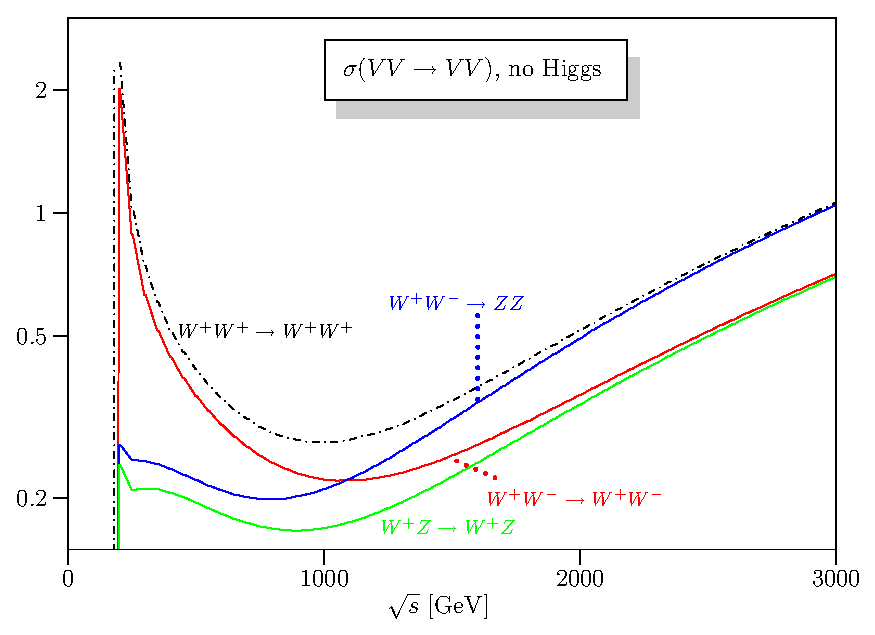
\includegraphics[width=0.48\textwidth]{standardModel/logres_noalphas_nohiggs.eps}
    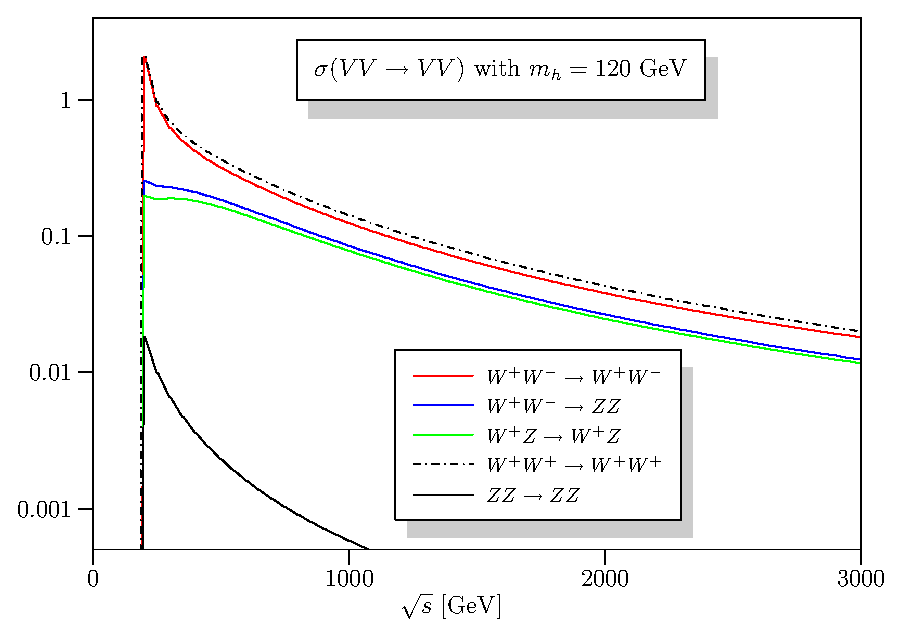
\includegraphics[width=0.48\textwidth]{standardModel/logres_noalphas_h120.eps}
    \caption[Unitarity violation in vector boson scattering without a Higgs boson]{
        $\PV\PV \to \PV\PV$ scattering cross sections as a function of center-of-mass energy for the SM with no Higgs boson (left) and a Higgs boson with $m_\PH = 120\GeV$ (right), reproduced from Ref.~\cite{Alboteanu:2008my}.
        The model with no Higgs violates unitarity.
      }\label{fig:vbsUnitarity}
  \end{center}
\end{figure}



\section{Limitations and Possible Extensions}

As noted above, the SM is believed to be fully self-consistent, but it has a number of notable omissions.
It makes no mention of gravity, which is too weak to be probed at the level of individual particles at energies available in today's collider experiments---or any collider experiment in the foreseeable future.
Neutrinos in the SM are massless, but they are found experimentally to oscillate between the three flavors in flight, which implies that the flavor eigenstates are not mass eigenstates, and thus that they have mass.
Dark matter is also not described.
Some consider the SM to be ``ad hoc'' in the sense that the fermion masses, and a number of other parameters---19 in all---are completely unconstrained, and a more aesthetically satisfying theory would make predictions for all of them.

A number of theories have been proposed which modify or extend the SM, adding new symmetry groups, unifying the existing ones further, adding new particles, etc.
A fourth generation of fermions would be a simple extension, but the fourth neutrino would have to have a mass more than half the {\PZ} boson mass to have escaped detection so far, which would be surprising given the small masses of the first three.
Supersymmetric models, for example, posit a symmetry between bosons and fermions, such that each particle would have a ``superpartner'' with the opposite spin statistics.
Despite extensive searches, no evidence of such models has been observed.
Another simple extension would be a new force, with mediator gauge bosons analogous to the {\PW} and {\PZ} above the masses accessible at existing colliders.
This, and several other possible extensions to the SM, would appear in practice as small deviations from the expected couplings of the gauge bosons.


\subsection{Anomalous Gauge Couplings}

Such deviations from standard model interactions are called anomalous gauge couplings (aGC), and may involve anomalous trilinear (aTGC) or quartic (aQGC) vertices.
Of particular interest here are the anomalous neutral couplings, which correspond to the vertices shown in Fig.~\ref{fig:aGCVertices}.
These interactions are forbidden in the SM\@.
Their existence would increase the cross section for diboson production, and affect the cross section for $\ZZ \to \ZZ$ scattering, changing the requirements on the Higgs field needed to preserve unitarity.

\begin{figure}[htbp]
  \vspace{1em}
  \begin{center}
    \begin{fmffile}{aTGCNeutral}
      \begin{fmfgraph*}(0.2,0.2) % chktex 36
        \fmfstraight %chktex 1
        \fmftop{d1,e1,d2}
        \fmfbottom{e2,d3,e3}
        \fmflabel{{\Pa}, {\PZ}}{e1}
        \fmflabel{{\Pa}, {\PZ}}{e2}
        \fmflabel{{\Pa}, {\PZ}}{e3}
        \fmf{zigzag}{e1,v1,e2}
        \fmf{zigzag}{v1,e3}
      \end{fmfgraph*}
    \end{fmffile}
    \hspace{4em}
    \begin{fmffile}{aQGCNeutral}
      \begin{fmfgraph*}(0.2,0.2) % chktex 36
        \fmfstraight %chktex 1
        \fmfleft{e1,e2}
        \fmfright{e3,e4}
        \fmflabel{{\Pa}, {\PZ}}{e1}
        \fmflabel{{\Pa}, {\PZ}}{e2}
        \fmflabel{{\Pa}, {\PZ}}{e3}
        \fmflabel{{\Pa}, {\PZ}}{e4}
        \fmf{zigzag}{e1,v1,e2}
        \fmf{zigzag}{e3,v1,e4}
      \end{fmfgraph*}
    \end{fmffile}
    \vspace{1em}
    \caption[Neutral anomalous gauge coupling vertices]{
        Fully-neutral gauge coupling vertices, for aTGCs (left) and aQGCs (right).
        These are forbidden in the SM\@.
      }\label{fig:aGCVertices}
  \end{center}
\end{figure}

Several theoretical frameworks exist for describing aGCs.
For aTGCs, we use the effective Lagrangian approach described in Ref.~\cite{Hagiwara:1986vm,Gounaris:2000tb,Baur:2000ae}.
In this parameterization, a $\PZ\PZ\PV$ coupling (where {\PV} may be {\PZ} or {\Pa}) has a vertex function corresponding to the vertex shown in Fig.~\ref{fig:aTGCLabels} of the form
\begin{equation}\label{eq:aTGCParam}
  \Gamma_\PV^{\alpha,\beta,\delta}\left(q_1,q_2,P\right) = i \frac{\hat{s} - m_\PV^2}{m_\PZ^2} \left(f_4^\PV \left(P^\alpha g^{\delta\beta} + P^\beta g^{\delta\alpha}\right) + f_5^\PV \varepsilon^{\delta\alpha\beta\lambda} \left(q_1 - q_2\right)_\lambda \right),
\end{equation}
where $\hat{s}$ is the center of mass energy squared, $g^{\mu\nu}$ is the Minkowski metric and $\varepsilon^{\alpha\beta\gamma\delta}$ is the fully antisymmetric tensor with $\varepsilon^{0123}=1$.
Neutral aTGCs are then described by two parameters $f_4^{\Pa,\PZ}$ associated to CP-odd terms and two parameters $f_5^{\Pa,\PZ}$ associated to CP-even terms.\footnote{There are, of course, analogous terms for all anomalous {\VVV} couplings, where {\PV} may be any of the electroweak bosons, but only the {\ZZZ} and $\ZZ\Pa$ terms are relevant to this work.}
The effective Lagrangians in use here are taken to be low-energy approximations invalid had high energy, and are not unitary at high $\sqrt{\hat{s}}$.
In some previous literature, unitarity is enforced with a generalized dipole for factor~\cite{Baur:1992cd,Baur:2000ae}, such that the vertex factor takes an energy dependence,
\begin{equation}
  f_i^\PV\left(\hat{s}\right) = \frac{f_{i,0}^\PV}{(1 + \hat{s} / \Lambda^2)^n},
\end{equation}
where $\Lambda$ is the energy scale of the new physics process.
No such form factor is applied in this work, to avoid adding unnecessary model dependence, so $\Lambda$ is taken to be much larger than the energies accessible in the experiment and no form factor is applied.

\begin{figure}[htbp]
  \vspace{1em}
  \begin{center}
    \begin{fmffile}{aTGCLabels}
      \begin{fmfgraph*}(0.25,0.25) % chktex 36
        \fmfstraight %chktex 1
        \fmfleft{d1,i1,d2}
        \fmfright{o1,d3,o2}
        \fmflabel{$V_\delta(P)$}{i1}
        \fmflabel{$Z_\alpha(q_1)$}{o1}
        \fmflabel{$Z_\beta(q_2)$}{o2}
        \fmf{zigzag}{o1,v1,o2}
        \fmf{boson}{i1,v1}
        \fmfblob{0.15w}{v1}
      \end{fmfgraph*}
    \end{fmffile}
    \vspace{1em}
    \caption[Neutral anomalous triple gauge coupling vertex]{
        An anomalous neutral triple gauge coupling vertex, with momentum labels corresponding to Eq.~(\ref{eq:aTGCParam}).
      }\label{fig:aTGCLabels}
  \end{center}
\end{figure}

For aQGCs, we adopt an effective field theory approach~\cite{Degrande:2012wf} which parameterizes the effects of new physics as a set of field operators~\cite{Eboli:2006wa}.
The operators are chosen to be dimension-8, because this is the lowest dimension that yields a theory with aQGCs but no aTGCs.
Out of the large class of operators which control aQGCs in general, {\ZZ} VBS is sensitive to five,
\begin{equation}
  \begin{aligned}
    \mathcal{L}_\text{T0} = & \frac{f_\text{T0}}{\Lambda^4} \text{Tr}\left[\hat{W}_{\mu\nu} \hat{W}^{\mu\nu}\right] \times \text{Tr}\left[\hat{W}_{\alpha\beta} \hat{W}^{\alpha\beta}\right] \\
    \mathcal{L}_\text{T1} = & \frac{f_\text{T1}}{\Lambda^4} \text{Tr}\left[\hat{W}_{\alpha\nu} \hat{W}^{\mu\beta}\right] \times \text{Tr}\left[\hat{W}_{\mu\beta} \hat{W}^{\alpha\nu}\right] \\
    \mathcal{L}_\text{T2} = & \frac{f_\text{T2}}{\Lambda^4} \text{Tr}\left[\hat{W}_{\alpha\mu} \hat{W}^{\mu\beta}\right] \times \text{Tr}\left[\hat{W}_{\beta\nu} \hat{W}^{\nu\alpha}\right] \\
    \mathcal{L}_\text{T8} = & \frac{f_\text{T8}}{\Lambda^4} B_{\mu\nu}B^{\mu\nu} B_{\alpha\beta}B^{\alpha\beta} \\
    \mathcal{L}_\text{T8} = & \frac{f_\text{T9}}{\Lambda^4} B_{\alpha\mu}B^{\mu\beta} B_{\beta\nu}B^{\nu\alpha},
  \end{aligned}
\end{equation}
where
\begin{equation}
  \hat{W}_{\mu\nu} = \sum_j W_{\mu\nu}^j \frac{\sigma^j}{2},
\end{equation}
and $\Lambda \gg \hat{s}$ is again the scale of the new physics causing the change in the effective couplings.



\section{Proton-Proton Collisions}\label{sec:pp}

Our experimental probe of all these interactions is proton-proton collisions.
As discussed above, protons are bound states of three quarks ($\Pqu\Pqu\Pqd$), known as the valence quarks, held together by virtual gluon exchange.
The proton constituents, quarks and gluons, are collectively called partons.
The gluons carry roughly half the total proton momentum~\cite{Halzen:1984mc}.
Because the number of gluons is not conserved, and they self-interact, the gluon structure of the proton is constantly evolving, and gluons produce virtual $\Pq\Paq$ ``sea quark'' pairs which annihilate again on time scales of order $t_\textit{virt} \sim 1 / \Delta E$~\cite{barger1997collider}.
A sufficiently energetic color-charged particle colliding with a proton may therefore interact with any kind of quark or with a gluon, and interesting physics in a {\pp} collision may be initiated by $\Pq\Pq, \Pq\Paq, \Pq\Pg$, or $\Pg\Pg$ scattering.
A particle that scatters with a proton of energy $P$ has a probability of interacting with a parton of a given type with momentum $xP$ given by the parton distribution function (PDF) $f(x,Q^2)$, where $Q$ is the momentum transfer of the interaction.
Heuristically, the PDF is a function of $Q$ because it sets the wavelength of the mediating gauge boson and thus the scale on which the interaction can resolve constituent partons.
PDFs are nonperturbative and cannot be calculated from theory, and are built from fits to experimental data from fixed-target and symmetric $\Pe^\pm\Pp$ deep inelastic scattering (DIS) data, and from hadron collider data~\cite{Ball:2017nwa}.
The most recent PDFs from the NNPDF collaboration are shown in Fig~\ref{fig:nnpdf}.

\begin{figure}[htbp]
  \begin{center}
    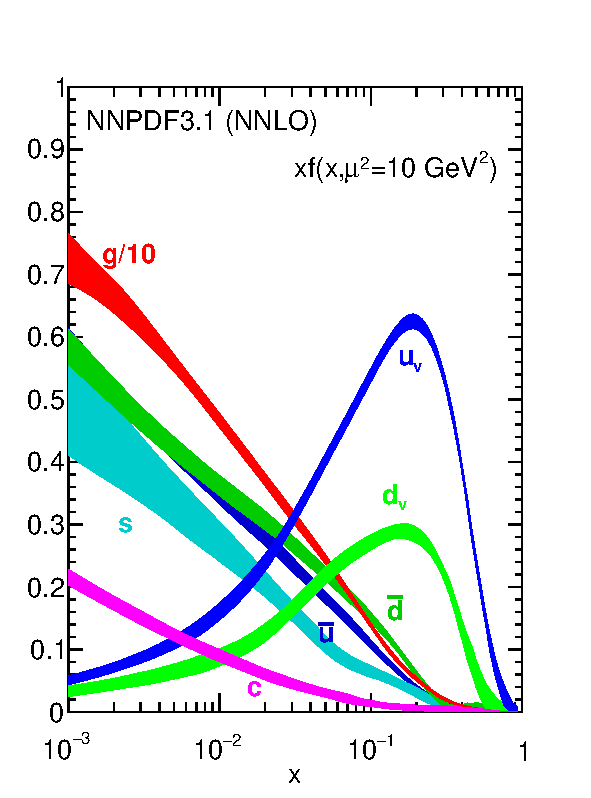
\includegraphics[width=0.48\textwidth]{standardModel/nnpdf31nnlo-10.pdf}
    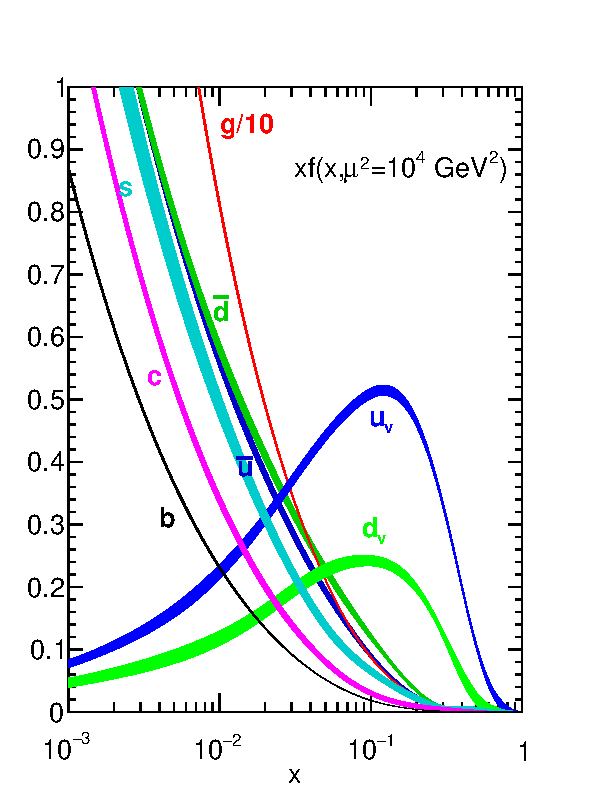
\includegraphics[width=0.48\textwidth]{standardModel/nnpdf31nnlo-1e4.pdf}
    \caption[Parton distribution functions]{
        Parton distribution functions from NNPDF3.1, reproduced from Ref.~\cite{Ball:2017nwa}, which used $\mu$ for the momentum transfer denoted $Q$ here.
      }\label{fig:nnpdf}
  \end{center}
\end{figure}

As mentioned previously, the rate at which a scattering process occurs is called its cross section $\sigma$, typically given barns, a unit of area $\unit{b} = 10^{-24}\unit{cm}^2$.
The number of collisions is characterized by the luminosity {\lumiL} such that the rate of events with final state $X$ will be given by
\begin{equation}
  \dd{N_X}{t} = \sigma\left(\pp \to X\right)\lumiL
\end{equation}
as described in more detail in Section~\ref{sec:lhc}.
If the initial protons each have momentum $P$ and collide head on, such that their center-of-mass energy is $\sqrt{s} = 2P$, the interacting partons will have total energy $\sqrt{\hat{s}} = \sqrt{2 x_1 x_2}P$ where $x_1$ and $x_2$ are the fraction of its proton's momentum each incoming parton carried.
The cross section is given by
\begin{equation}
  \sigma\left(\pp \to X\right) = \sum_{p_1,p_2 \in \Pq, \Paq, \Pg} C_{p_1,p_2} \int \cmsSymbolFace{d}x_1 \cmsSymbolFace{d}x_2 f_{p_1}(x_1,Q^2) f_{p_2}(x_2,Q^2) \sigma_\text{ME}(p_1+p_2 \to X),
\end{equation}
where $\sigma_\text{ME}$ is the matrix element-level cross section for the bare partons to scatter to final state $X$ and $C_{p_1,p_2}$ is a combinatoric factor based on the number of possible color combinations that varies based on the initial state particles $p_1$ and $p_2$.
This factorization into perturbative hard process physics and the nonperturbative PDF greatly simplifies calculaitons.



\section{Topics Covered In This Thesis} % chktex 17
